%latex main.tex
%bibtex main
%latex main.tex
%latex main.tex
%dvipdfm main.dvi

%se poate lucra si online (de ex www.overleaf.com)


\documentclass[runningheads,a4paper,11pt]{report}

\usepackage{algorithmic}
\usepackage{algorithm} 
\usepackage{array}
\usepackage{amsmath}
\usepackage{amsfonts}
\usepackage{amssymb}
\usepackage{amsthm}
\usepackage{caption}
\usepackage{comment} 
\usepackage{epsfig} 
\usepackage{fancyhdr}
\usepackage[T1]{fontenc}
\usepackage{geometry} 
\usepackage{graphicx}
\usepackage[colorlinks]{hyperref} 
\usepackage[latin1]{inputenc}
\usepackage{multicol}
\usepackage{multirow} 
\usepackage{rotating}
\usepackage{setspace}
\usepackage{subfigure}
\usepackage{url}
\usepackage{verbatim}
\usepackage{xcolor}

\geometry{a4paper,top=3cm,left=2cm,right=2cm,bottom=3cm}

\pagestyle{fancy}
\fancyhf{}
\fancyhead[LE,RO]{Project's name}
\fancyhead[RE,LO]{Team's name}
\fancyfoot[RE,LO]{MIRPR 2019-2020}
\fancyfoot[LE,RO]{\thepage}

\renewcommand{\headrulewidth}{2pt}
\renewcommand{\footrulewidth}{1pt}
\renewcommand{\headrule}{\hbox to\headwidth{%
  \color{lime}\leaders\hrule height \headrulewidth\hfill}}
\renewcommand{\footrule}{\hbox to\headwidth{%
  \color{lime}\leaders\hrule height \footrulewidth\hfill}}

\hypersetup{
pdftitle={artTitle},
pdfauthor={name},
pdfkeywords={pdf, latex, tex, ps2pdf, dvipdfm, pdflatex},
bookmarksnumbered,
pdfstartview={FitH},
urlcolor=cyan,
colorlinks=true,
linkcolor=red,
citecolor=green,
}
% \pagestyle{plain}

\setcounter{secnumdepth}{3}
\setcounter{tocdepth}{3}

\linespread{1}

% \pagestyle{myheadings}

\makeindex


\begin{document}

\begin{titlepage}
\sloppy
\begin{center}
BABE\c S BOLYAI UNIVERSITY, CLUJ NAPOCA, ROM\^ ANIA

FACULTY OF MATHEMATICS AND COMPUTER SCIENCE

\vspace{6cm}

\Huge \textbf{PEDESTRIAN DETECTION}

\vspace{1cm}

\normalsize -- MIRPR report --

\end{center}


\vspace{5cm}

\begin{flushright}
\Large{\textbf{Team members}}\\
Name, specialisation, group \\
Jurj Flaviu Andrei, informatics in english, 934 \\
Maxim Tudor, informatics in english, 934 \\
Moisi Teofana Ionela, informatics in english, 934 \\
\end{flushright}

\vspace{4cm}

\begin{center}
2019
\end{center}

\end{titlepage}

\pagenumbering{gobble}

\begin{abstract}
	Text of abstract. Short info about: project relevance/importance, inteligent methods used for solving, data involved in the numerical experiments; conclude by the the results obtained. \\

	Designing autonomous vehicles for the diverse urban traffic remains an unresolved problem due to its large number of events both expected and unexpected requiring various actions in a very short amount of time. In the recent years, major improvements were achieved, but we are still very far from the moment where the set of algorithms and techniques would be able to replace the human driver. \\

	Object detection represents a major topic in the goal of addressing the issue of autonomous vehicles and more specifically pedestrian detection is a complex task due to its high variety of factors and challenges such as various height, weight, clothing, frequent occlusion between pedestrians etc. We are going two intelligent methods in order to solve this problem and we will compare the results based on some benchmarks. \\

	The data involved will be gathered from previously constructed and approved datasets consisting of frames(images) or short-length clips which will be further decomposed in frames.
\end{abstract}


\tableofcontents

\newpage

\listoftables
\listoffigures
\listofalgorithms

\newpage

\setstretch{1.5}



\newpage

\pagenumbering{arabic}


 


\chapter{Introduction}
\label{chapter:introduction}

\section{What? Why? How?}
\label{section:what}

Motivate and abstractly describe the problem you are addressing and how you are addressing it. 
\begin{itemize}
	\item What is the (scientific) problem? 
	\begin{itemize}
		\item The pedestrian detection task represents a special case of object detection being related to computer vision and image processing. From an intelligent algorithm perspective, we can say that it represents a classification problem.
	\end{itemize}
	\item Why is it important? 
	\begin{itemize}
		\item Pedestrian detection represents one of the core functionalities necessary for an autonomous vehicle. Moreover, the detection must be both reliable and fast taking into consideration all the possible factors which can occur.
	\end{itemize}
	\item What is your basic approach? 
	\begin{itemize}
		\item $\ldots$ \#TODO
	\end{itemize}
\end{itemize}

Pedestrian detection represents one of the well-researched domains of object detection alongside face recognition.Consequently, many perspective were checked during its life course and non-intelligent solutions were found unsufficient for the variety of factors which should be taken into consideration. We are going to use and compare two different intelligent methods which will hopefully improve previous research on the topic.


\section{Paper structure and original contribution(s)}
\label{section:structure}

The research presented in this paper advances the theory, design, and implementation of several particular mains. 

The main contribution of this report is to present an intelligent algorithm for solving the problem of \textbf{pedestrian detection}.

The second contribution of this report consists of building an intuitive, easy-to-use and user
friendly software application. Our aim is to build an algorithm that will help both car makers for further improvements to the automated driving system and casual drivers with live alerts in the traffic

The third contribution of this thesis consists of $\ldots$.


The present work contains $xyz$ bibliographical references and is structured in five chapters as follows.

The first chapter/section is a short introduction in the problem of pedestrian detection.

The second chapter/section describes the scientific problem and the approaches used to solve it.

The chapter/section \ref{chapter:proposedApproach} details $\ldots$.



\chapter{Scientific Problem}
\label{section:scientificProblem}


\section{Problem definition}
\label{section:problemDefinition}

Give a description of the problem.
Explain why it must be solved by an intelligent algorithm. 
Details the advantages and/or disadvantages of solving the problem by a (some) given method(s).

Precisely define the problem you are addressing (i.e. formally specify the inputs and outputs). Elaborate on why this is an interesting and important problem.


Object detection has been a trending topic in the recent years due to innovation in intelligent methods, but also in hardware performance. Pedestrian detection represents a canonical sub-problem with diverse applications, the main one being autonomous driving. Despite the extensive research on this particular problem, recent papers still show significant improvements over older ones while still being far from the accuracy of a human.To cite a recent piece of research will evaluated the best methods available: "The results indicate that there is still a ten fold improvement to be made before reaching human performance." \\
The presented problem is really complex due to its high variety of factors and challenges such as different height, weight, clothing, frequent occlusion betweend pedestrians etc. Consequently, c onvential non-intelligent methods constructed in the past were found to be insufficient to solve the problem in a generalized manner, being only very accurate on specific cases and environments. As a result, the trend has shifted towards variations of intelligent algorithms which may generalize more easily the problem while maintaining ideas from the specific implementations.

Since the topic consists mostly in the analysis of visual images, the usage of convolutional neural network with their variations has been a major player in the recent time. The advantages of this method stems from the fact that these types of networks tend to learn by themselves which filters are relevant for the specific problem, eliminating the need to hand-engineer them like in traditional algorithms of image classification. One major disadvantage represents the need for a relatively large training data set which isn't always available.



The inputs for this problem might be of two types: images and short clips, the later one being converted into a set of relevant frames which will be interpreted as normal images. The resolution among the input data should be kept consistent in order to ensure the correctitude of the evaluation. Otherwise, different methods of rescaling should be used, while maintaining the original details: as little distortion, blur and noise as possible. \\
The main outputs of the application will be classified images where each pedestrian will be bounded with a box in order to denote its position. Moreover, we may generate secondary textual outputs which will contain only the relevant information found by the intelligent algorithm: the corners coordinates for the boxes.



Item example: 

\begin{itemize}
	\item content of item1
 	\item content of item2
 	\item content of item3
\end{itemize}



Figure example 

$\ldots$ (see Figure \ref{swarmsize})

\begin{figure}[htbp]
	\centerline{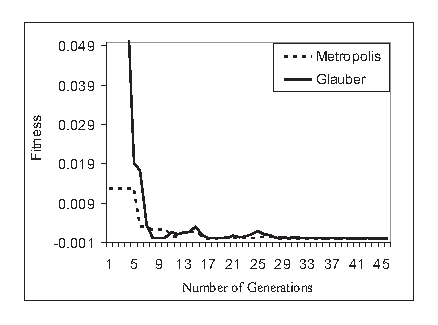
\includegraphics{Fig/FitEvol.eps}}  
	\caption{The evolution of the swarm size during the GA generations. This results were obtained for the $f_2$ test function with 5 dimensions.}
	\label{swarmsize}
\end{figure}


Table example: (see Table \ref{tab3PSO})


\begin{table}[htbp]
	\caption{The parameters of the PSO algorithm (the micro level algorithm) used to compute the fitness of a GA chromosome.}
	\label{tab3PSO}
		\begin{center}
			\begin{tabular}{p{220pt}c}

				\textbf{Parameter}& \textbf{Value} \\
				\hline\hline
 				Number of generations& 50 \\
 				Number of function evaluations/generation& 10 \\
 				Number of dimensions of the function to be optimized& 5 \\
 				Learning factor $c_{1}$& 2 \\
 				Learning factor $c_{2}$ & 1.8\\
 				Inertia weight& 0.5 + $\frac{rand()}{2}$\\
		
			\end{tabular}
		\end{center}
\end{table}

Algorithm example 

$\ldots$ (see Algorithm \ref{NGalg})


\algsetup{indent=1em, linenosize=\footnotesize}

\begin{algorithm}
	\caption{SGA - Spin based Genetic AQlgorithm}
	\label{NGalg}
		\begin{algorithmic}


			\STATE \textbf{BEGIN}
  		\STATE @ Randomly create the initial GA population.
  		\STATE @ Compute the fitness of each individual.
  		\FOR{i=1 TO NoOfGenerations}
  			\FOR{j=1 TO PopulationSize}
  				\STATE p $\leftarrow$ RandomlySelectParticleFromGrid();
  				\STATE n $\leftarrow$ RandomlySelectParticleFromNeighbors(p);
  				\STATE @ Crossover(p, n, off);
  				\STATE @ Compute energy $\Delta H$
  				\IF {$\Delta H$ satisfy the Ising condition}
  					\STATE @ Replace(p,off);
  				\ENDIF
  			\ENDFOR
  		\ENDFOR
  		\STATE \textbf{END}
\end{algorithmic}
\end{algorithm}


\chapter{State of art/Related work}
\label{chapter:stateOfArt}


The theory of the methods utilised until now in order to solve the given problem.

Answer the following questions for each piece of related work that addresses the same or a similar problem. 
\begin{itemize}
	\item What is their problem and method? 
	\item How is your problem and method different? 
	\item Why is your problem and method better?
\end{itemize} 



\textbf{Detecting Pedestrians by Learning Shapelet Features} \\
Payam Sabzmeydani and Greg Mori \\
School of Computing Science Simon Fraser University \\

\begin{itemize}
	\item What is their problem and method?	
	\begin{itemize}	
		\item They approach the problem of pedestrians detection in still images. They use AdaBoost training algorithm for face and pedestrians classification on the MIT and INRIA datasets.
			A major drawback is the fixed set of feature descriptors  and the problem with defining them is that there could be some discriminative information that is missed by those features . For training, they use three steps: low-level features, shapelet features and the final classifier.
	\end{itemize}
	\item How is your problem and method different?	
	\begin{itemize}
		\item Our aim is the same: to find a method to detect the pedestrians in the most accurate way. Besides detecting wether there are or not pedestrians, we would like to see how close they are. 
	We will use TensorFlow and compare the results afterwards and also use different datasets. 
	Another option is to use the AdaBoost training algorithm as well and try to change the training features and final classifier, in order to get better results, bu comparison.
	They compare their results with HOG-SVM detector of Dalal and Triggs and maybe we could find another detector results to compare with.
	\end{itemize}
	\item Why is your problem and method better?	
	\begin{itemize}
		\item Detecting how close we are to the pedestrians could be an improvement besides detecting wether there are pedestrians or not.
	\end{itemize}
\end{itemize}


\textbf{Pedestrian Detection: A Benchmark} \\
Piotr Dollar, Christian Wojek, Bernt Schiele, Pietro Perona \\

1. What is their problem and method?  \\
Pedestrian detection represents a key problem in computer vision and most of the recent important evolution in this field has been realized thanks to the challenging public datasets. They come with the new dataset: Caltech Pedestrians Dataset, which is two times larger than the existing ones. They propose improved performance metrics and they benchmark 7 algorithms. Moreover, they classify the pedestrians by the distance from the camera: near, medium and far. \\

2. How is your problem and method different? \\ 
Our problem resumes basically to the same thing and we will try to obtain similar results using other methods and algorithms. We are going to use implement a neuronal network using TensorFlow and see how our results will differ. \\

3. Why is your problem and method better? \\
We are going to work on more datasets, so that the images will vary more. We could also try to process short videos, not only images. \\



\textbf{Understanding Pedestrian Behavior in Complex Traffic Scenes} \\
	Amir Rasouli, Iuliia Kotseruba, and John K. Tsotsos \\

This piece of research aimed to identify, analyze and present the pedestrian behaviour in traffic from a moving car perspective. Its purpose was to evaluate the crossing patterns, how pedestrians communicate their intention and to find other factors which may influence the pedestrians decisions. \\
Consequently, they create a new dataset composed of short clips presenting possible events of crossing in different conditions. The data was annotated in two manners: bounding boxes representative for pedestrian detection and textual associated with behavioural data about the pedestrians and drivers actions and contextual information such as demographics, ambient conditions and environmental factors. Multiple labelers were used in order to minimize the subjective bias while assessing the data and some actions were removed from the dataset since there wasn't a consensus between the labelers. \\
The study evaluated many perspectives and found out some interesting remarks: \\
\begin{itemize}
	\item the context in which pedestrians are observed plays an important role along their position and head orientation, indicator of crossing intention;
	\item there are often used explicit means of communications to resolve conflicts in traffic scenes (e.g. handwaves, driver using the led lights)
	\item various elements in a scene such as width of the street, the presence of a zebra crossing or a traffic signal can greatly influence the pedestrian confidence of crossing, representing a valuable way to predict his further actions
	\item the driver's dynamic state with respect to the pedestrians influence their behaviour, Time-To-Collision being used as a representative factor
\end{itemize}
The study seems to suggest that there's also an interrelationship between various contextual elements which influence the pedestrian behaviour as a whole. There are more factors which can be furtherly studied such as environmental conditions (weather, light), social conditions and demographic conditions. Moreover, studies based on surveys should be conducted in order to fully eliminate subjectivity bias in determining and labeling pedestrians' intentions and actions. \\ 





\textbf{How Far are We from Solving Pedestrian Detection?} \\
	Shanshan Zhang, Rodrigo Benenson, Mohamed Omran, Jan Hosang and Bernt Schiele \\
	Max Planck Institute for Informatics \\
	Saarbrücken, Germany \\



	This piece of research goal was to improve the current best performers intelligent algorithms over the Caltech Dataset on pedestrian detection. In the last years, two categories of methods have been defined and chosen for their performance towards this topic: integral channel feature detector (ICF) and training convolution neural networks (convnets) for these specific types of images. \\
	The study compared previous implementations performance on the mentioned dataset to a proprietary variation of the original \textbf{Checkerboards} detector which furtherly is a generalisation of the Integral Channels Feature Detector (ICF). Their implementation called \textbf{Rotated Filters} decreased the number of filters used for training and being applied at three different scales. \\
	When it comes to convolution neural networks they compared  two of them: AlexNet and VGG16. Both used a subclass of convnets, called R-CNN (region convolution neural networks).In R-CNN the CNN is forced to focus on a single region at a time because that way interference is minimized because it is expected that only a single object of interest will dominate in a given region. The regions in the R-CNN are detected by selective search algorithm followed by resizing so that the regions are of equal size before they are fed to a CNN for classification and bounding box regression. These types of convnets are specifically designed for object detection from which pedestrian detection is part of. Based on their statistics, they found that the convnets have difficulties in evaluating windows surrounding true positivies especially when talking about small objects as dimension in the images. They hypothesise that the performance is a limitation on the tested convnets architecture which should be reconfigured to some which are closer to the ones used for semantic labelling or boundaries estimation tasks which require pixel-accurate output. \\
	We are going to take these suggestions into consideration when designing our convolution neural networks in order to improve their performance on a bigger variety of scenarious.




In order to cite a given work you can use a bib file (see the example) and the $\ $ \textit{cite} command:
\cite{kennedy1}, \cite{Koh06}, \cite{Berlekamp82}, \cite{Storn95}, \cite{firefox}.



\chapter{Proposed approach}
\label{chapter:proposedApproach}

Describe your approach!

Describe in reasonable detail the algorithm you are using to address this problem. A psuedocode description of the algorithm you are using is frequently useful. Trace through a concrete example, showing how your algorithm processes this example. The example should be complex enough to illustrate all of the important aspects of the problem but simple enough to be easily understood. If possible, an intuitively meaningful example is better than one with meaningless symbols.


\chapter{Application (numerical validation)}
\label{chapter:application}


Explain the experimental methodology and the numerical results obtained with your approach and the state of art approache(s).

Try to perform a comparison of several approaches.

Statistical validation of the results.


\section{Methodology}
\label{section:methodology}

\begin{itemize}
	\item What are criteria you are using to evaluate your method? 
	\item What specific hypotheses does your experiment test? Describe the experimental methodology that you used. 
	\item What are the dependent and independent variables? 
	\item What is the training/test data that was used, and why is it realistic or interesting? Exactly what performance data did you collect and how are you presenting and analyzing it? Comparisons to competing methods that address the same problem are particularly useful.
\end{itemize}

\section{Data}
\label{section:data}

Describe the used data.

\section{Results}
\label{section:results}

Present the quantitative results of your experiments. Graphical data presentation such as graphs and histograms are frequently better than tables. What are the basic differences revealed in the data. Are they statistically significant?

\section{Discussion}
\label{section:discussion}

\begin{itemize}
	\item Is your hypothesis supported? 
	\item What conclusions do the results support about the strengths and weaknesses of your method compared to other methods? 
	\item How can the results be explained in terms of the underlying properties of the algorithm and/or the data. 
\end{itemize}



\chapter{Conclusion and future work}
\label{chapter:concl}

Try to emphasise the strengths and the weaknesses of your approach.
What are the major shortcomings of your current method? For each shortcoming, propose additions or enhancements that would help overcome it. 

Briefly summarize the important results and conclusions presented in the paper. 

\begin{itemize}
	\item What are the most important points illustrated by your work? 
	\item How will your results improve future research and applications in the area? 
\end{itemize}


\bibliographystyle{plain}
\bibliography{BibAll}

\end{document}
